% Very simple template for lab reports. Most common packages are already included.
\documentclass[a4paper, 11pt]{article}
\usepackage[utf8]{inputenc} % Change according your file encoding
\usepackage{graphicx}
\usepackage{url}
\usepackage{listings}
\usepackage{xcolor}
\usepackage{float} % provide [H] placement to pin floats
\usepackage{placeins} % provide \FloatBarrier to prevent floats passing barriers


%opening
\title{Report 1: Rudy the HTTP Server}
\author{Lorenzo Deflorian}
\date{\today{}}

\begin{document}

\maketitle

\section{Introduction}

The main goal of this assignment was to implement a simple HTTP server in Erlang.
The server needed to accept socket connections, parse HTTP requests, and send responses.
Another important aspect was gaining a deeper understanding of Erlang processes and how to use them to handle multiple clients concurrently.
Finally, I evaluated the server's performance by comparing the different implementation approaches I explored.


\section{Main problems and solutions}

The first task was to create a simple HTTP server that could handle requests sequentially.
This was straightforward using the built-in \texttt{gen\_tcp} module for socket connections. After implementing the basic server, I benchmarked it to measure performance for 100 sequential requests.

\begin{verbatim}
  (client@DORORO)1> test:bench(localhost, 8080).
  Time Elapsed 174.338 ms
  ok
\end{verbatim}

Normalizing the elapsed time by the number of requests gives an average latency of 1.743 ms per request. Hence, the server can handle about 573 requests per second.

The next step was to add a small processing delay (40 ms) to simulate a more realistic scenario and see if the overhead given by the parsing of the request is significant.

\begin{verbatim}
  (client@DORORO)1> test:bench(localhost, 8080).
  Time Elapsed 4408.464 ms
  ok
\end{verbatim}

The artificial delay increases latency to 44 ms per request, showing that server overhead is negligible compared to processing time.

To improve performance, we implemented a concurrent approach that creates a new process for each incoming connection, allowing multiple requests to be handled in parallel. This raises the question: how lightweight are Erlang processes? To answer this, I implemented a concurrent version of the server to measure overhead from process creation.

\begin{table}[H]
\centering
\begin{tabular}{|l|c|}
\hline
\textbf{Metric} & \textbf{Time (ms)} \\
\hline
Average process creation time & 0.015 \\
Maximum process creation time & 0.171 \\
Minimum process creation time & 0.006 \\
\hline
\end{tabular}
\caption{Process creation time statistics}
\label{tab:process_creation_time}
\end{table}
\FloatBarrier

Table \ref{tab:process_creation_time} shows the average process creation time is about 0.015 ms, which is quite low. Therefore, we can create many processes without significant overhead.

\section{Evaluation}
\subsection{First concurrent implementation}

Let's evaluate the server's performance with multiple clients connected at the same time.
The server was launched with:
\begin{verbatim}
spawn_rudy:start(8080).  
\end{verbatim}
and the clients with (100 clients in total):
\begin{verbatim}
test:bench_many(100, "localhost", 8080).
\end{verbatim}

I got the following results:
\begin{figure}[H]
  \centering
  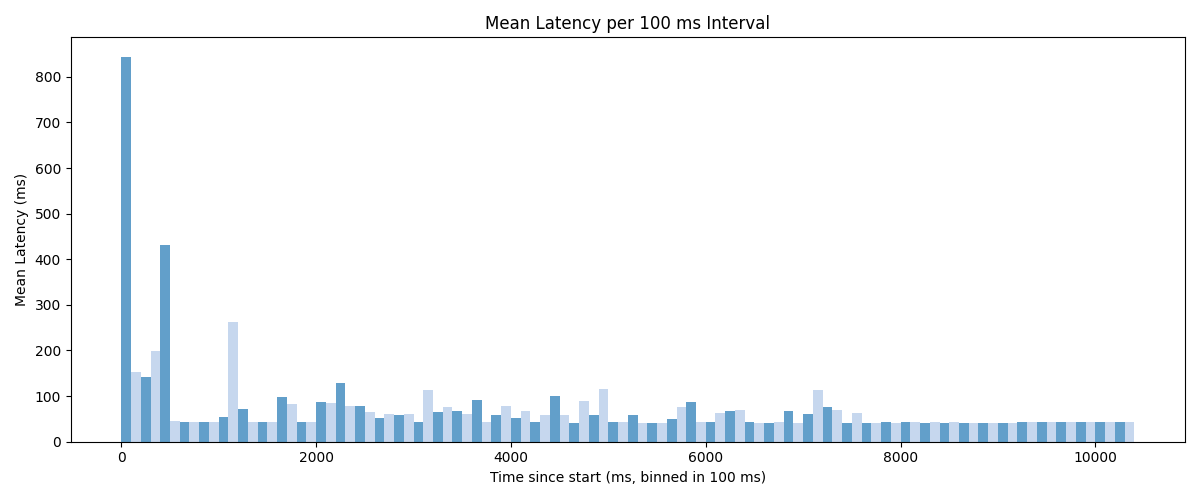
\includegraphics[width=0.9\linewidth]{many_benches/latency_histogram.png}
  \caption{Latency Histogram}
  \label{fig:latency_histogram}
\end{figure}
\FloatBarrier

As shown, Erlang can handle many requests concurrently with good performance. The initial spike in latency is due to the first requests being processed; as the server warms up, latency stabilizes at a lower value.

Overall, even with a very simple implementation, Erlang proves to be a powerful tool for building concurrent servers.

\subsection{Comparison between sequential and concurrent implementations}

We next evaluate a more stable approach and compare it to the initial sequential implementation.

The \texttt{multi\_rudy} implementation uses a pool of handlers to limit the number of concurrent processes and avoid overwhelming the system.

I benchmarked the sequential server using three clients and measured latency.

\begin{figure}[H]
  \centering
  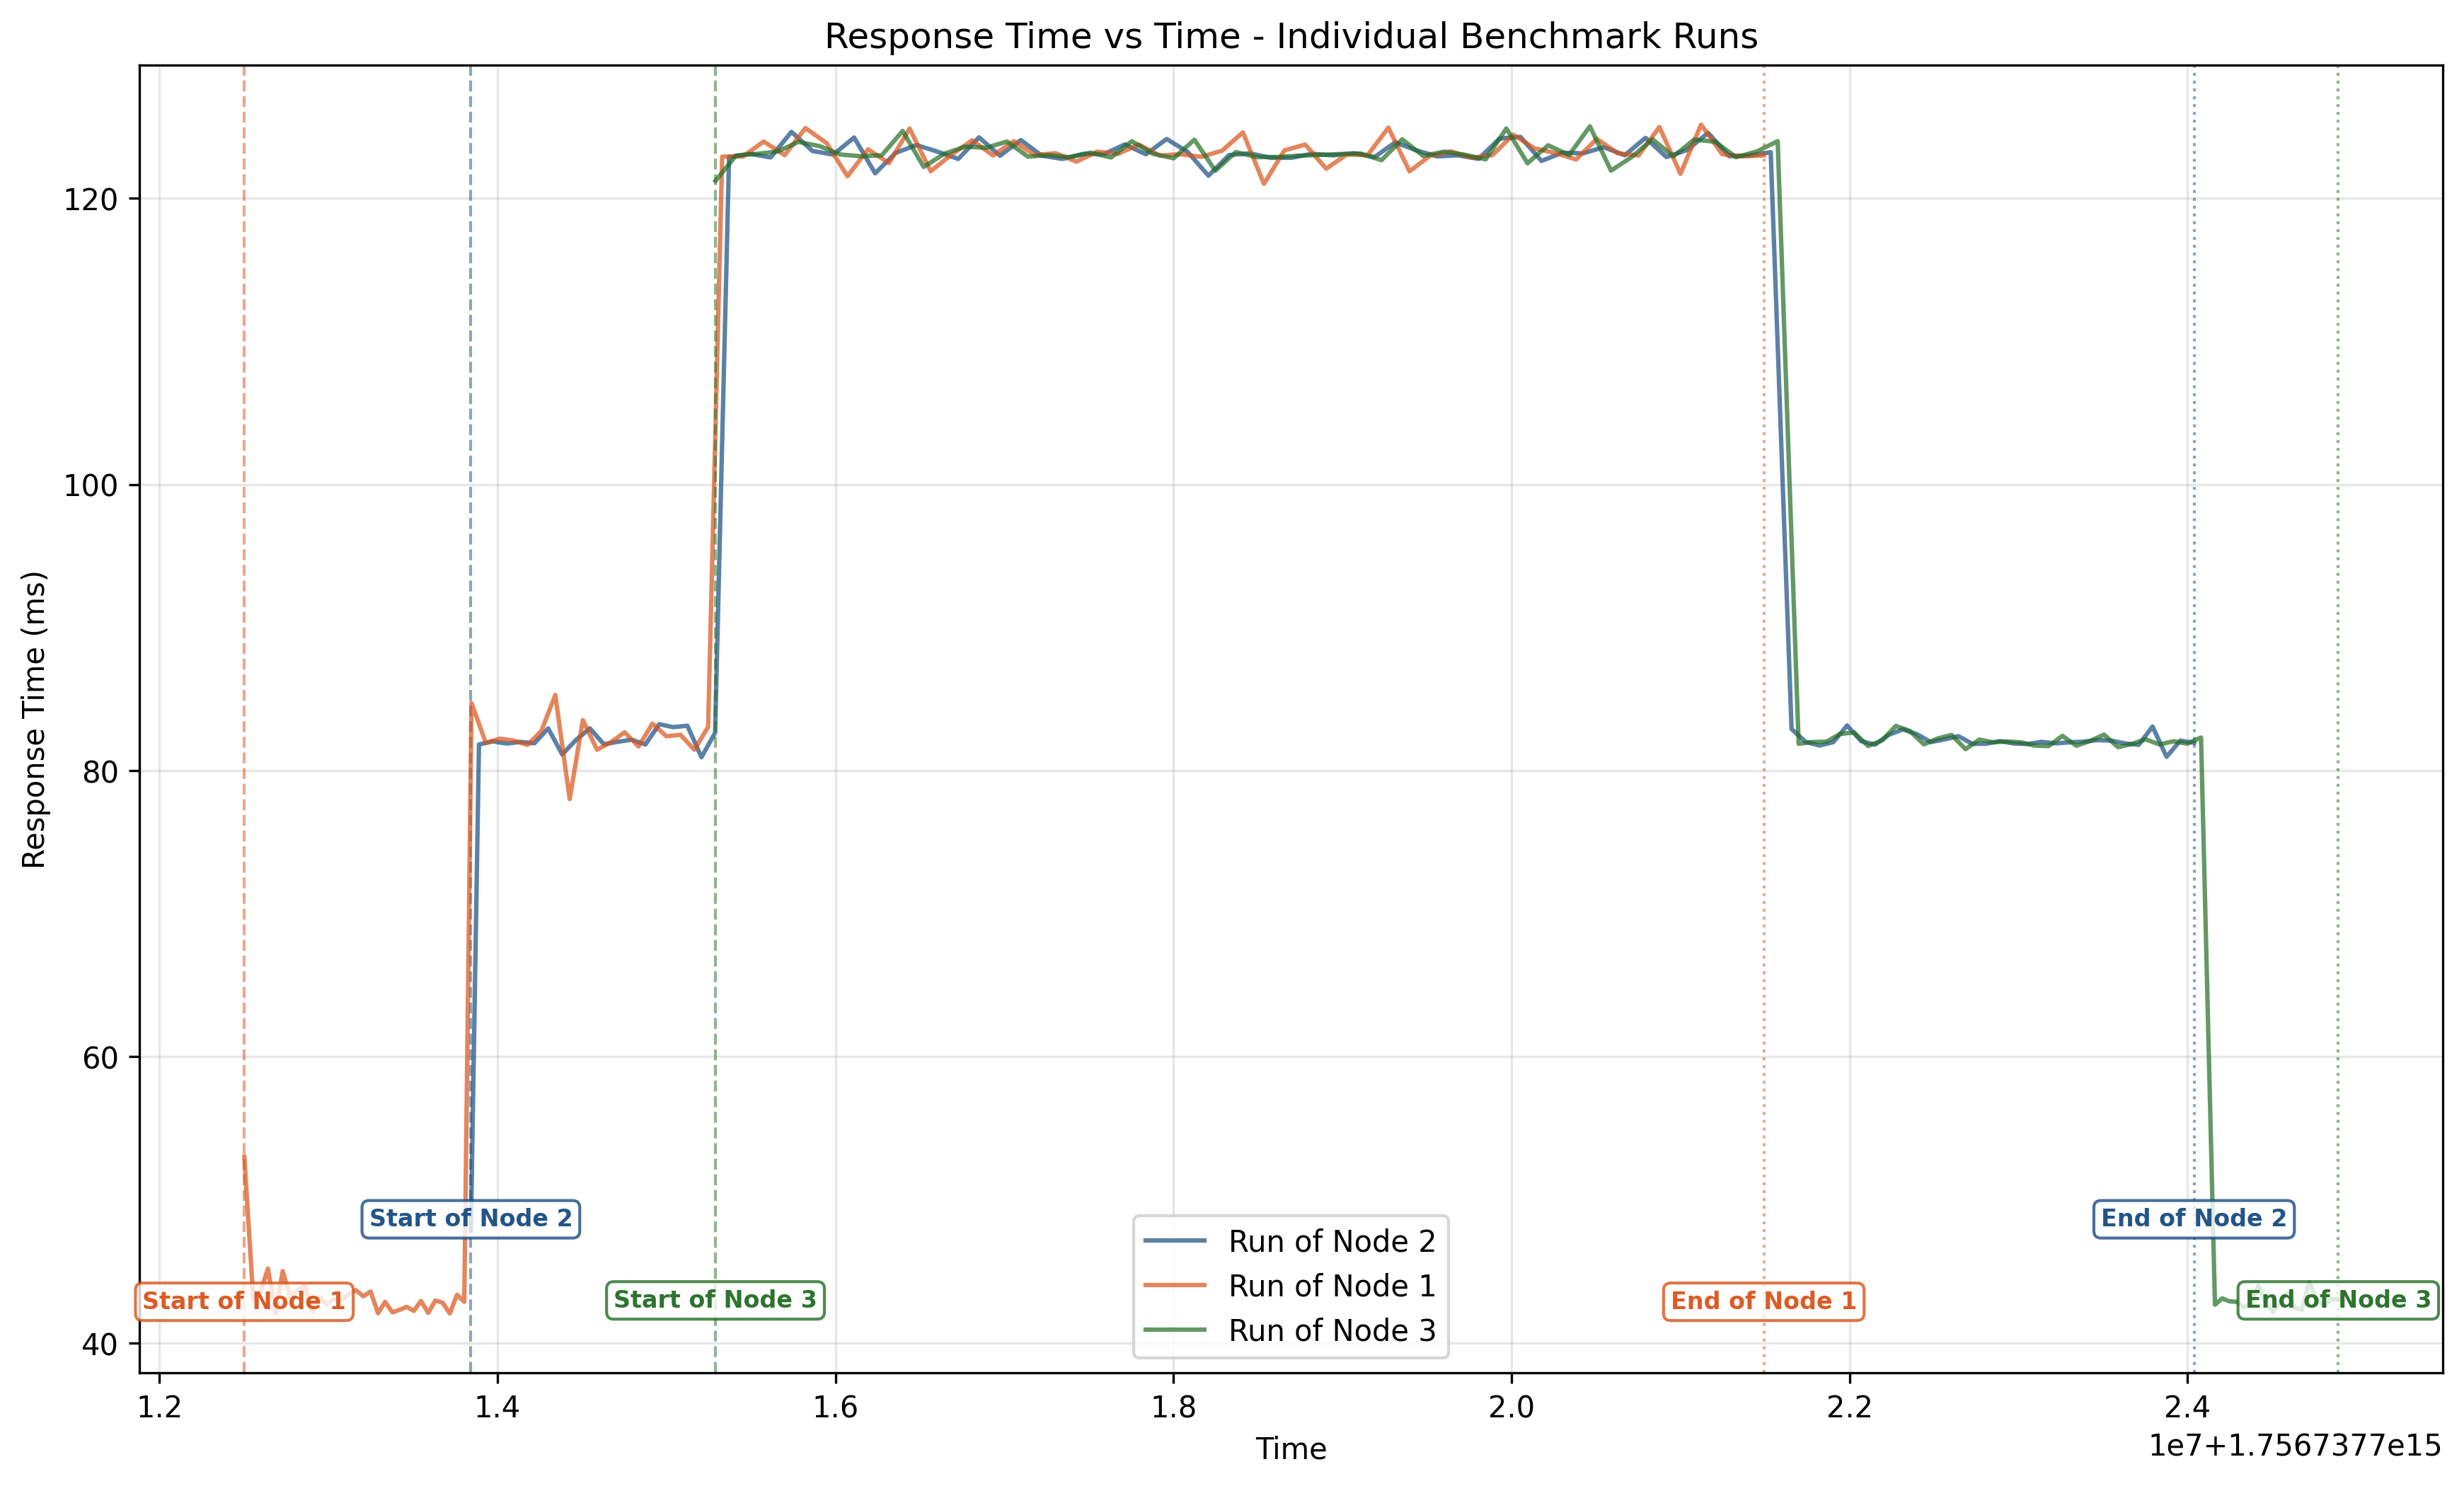
\includegraphics[width=0.9\linewidth]{sequential_benches/latency_plot.png}
  \caption{Latency Comparison (Sequential)}
  \label{fig:latency_comparison_seq}
\end{figure}
\FloatBarrier

Figure \ref{fig:latency_comparison_seq} shows that latency increases roughly linearly with the number of connected clients, as expected. Each time a client finishes its batch of requests, latency drops because fewer clients are connected to the server.

We now evaluate how the concurrent version performs.

\begin{figure}[H]
  \centering
  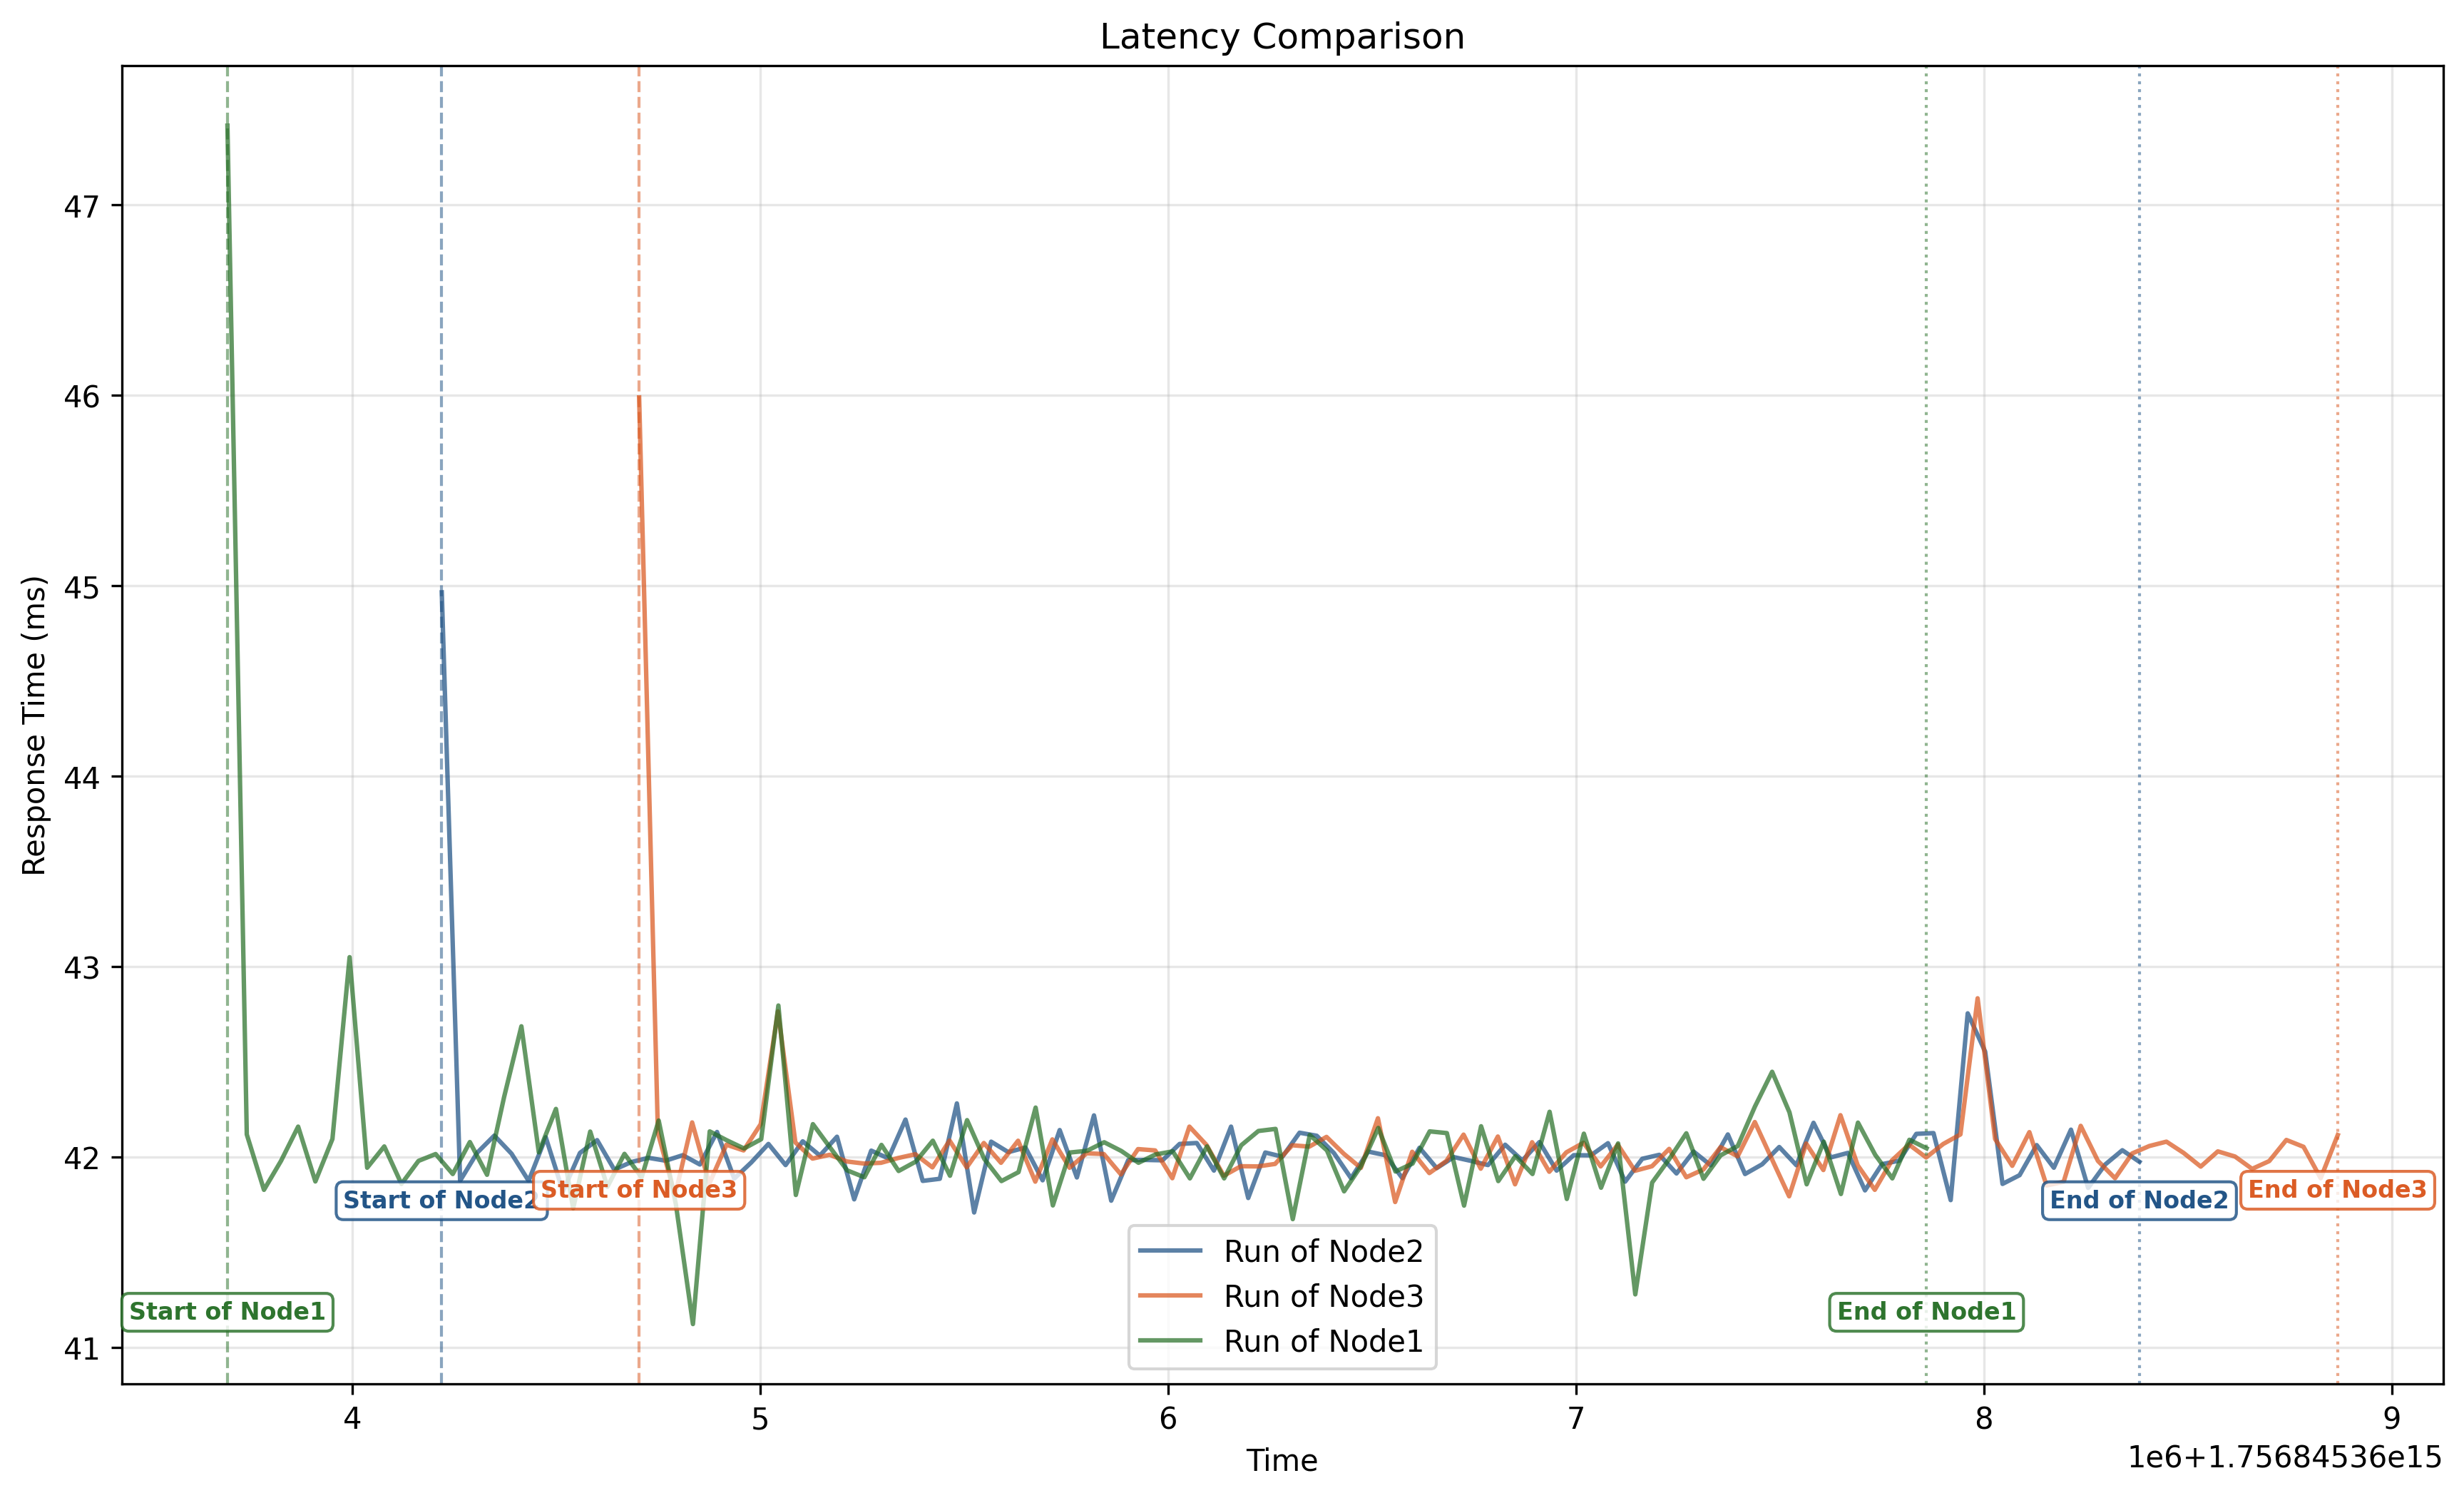
\includegraphics[width=0.9\linewidth]{concurrent_benches/latency_plot.png}
  \caption{Latency Comparison (Concurrent)}
  \label{fig:latency_comparison_conc}
\end{figure}
\FloatBarrier

The \texttt{multi\_rudy} implementation performs significantly better than the sequential version: because each handler processes requests independently, overall latency is much lower. We have increased throughput!


\section{Conclusions}

This report explored the performance of a simple sequential server implementation in Erlang and compared it with a concurrent version using a pool of handlers. We found that the sequential implementation suffers increased latency as the number of connected clients grows, while the concurrent implementation handles multiple requests in parallel with much lower latency.

\end{document}